%!TEX root = ../MCGT_Thesis.tex

%\begin{savequote}[8cm]
%\textlatin{Cor animalium, fundamentum e\longs t vitæ, princeps omnium, Microco\longs mi Sol, a quo omnis vegetatio dependet, vigor omnis \& robur emanat.}

%The heart of animals is the foundation of their life, the sovereign of everything within them, the sun of their microcosm, that upon which all growth depends, from which all power proceeds.
%  \qauthor{--- William Harvey \cite{harvey_exercitatio_1628}}
%\end{savequote}

\chapter{Background}
\label{ch:1-Background}
%\minitoc
Aliquet. Mattis vitae curae; pede rhoncus fermentum non. Hendrerit per Bibendum tristique volutpat massa vitae imperdiet nulla justo ullamcorper molestie tortor posuere porta auctor, egestas ullamcorper neque platea, hymenaeos suscipit. Primis vulputate.  \citep{world1992icd}.

\section{Characteristics of chronic pain}

\citet{breivik2006survey} Aliquet. Mattis vitae curae; pede rhoncus fermentum non. Hendrerit per Bibendum tristique volutpat massa vitae imperdiet nulla justo ullamcorper molestie tortor posuere porta auctor, egestas ullamcorper neque platea, hymenaeos suscipit. Primis vulputate.  (\citeyear{breivik2006survey}) Aliquet. Mattis vitae curae; pede rhoncus fermentum non. Hendrerit per Bibendum tristique volutpat massa vitae imperdiet nulla justo ullamcorper molestie tortor posuere porta auctor, egestas ullamcorper neque platea, hymenaeos suscipit. Primis vulputate. \citep{breivik2006survey}. Given these aetiologic and diagnostic differences, the ``typical'' chronic pain characteristics may be heterogeneous and may include highly physically disabled patients, fibromyalgia, chronic headache, rheumatoid arthritis, whiplash-associated disorders, muscoloskeletal disorder, chronic fatigue syndrome,  and others. 



 \begin{figure}
 	\centering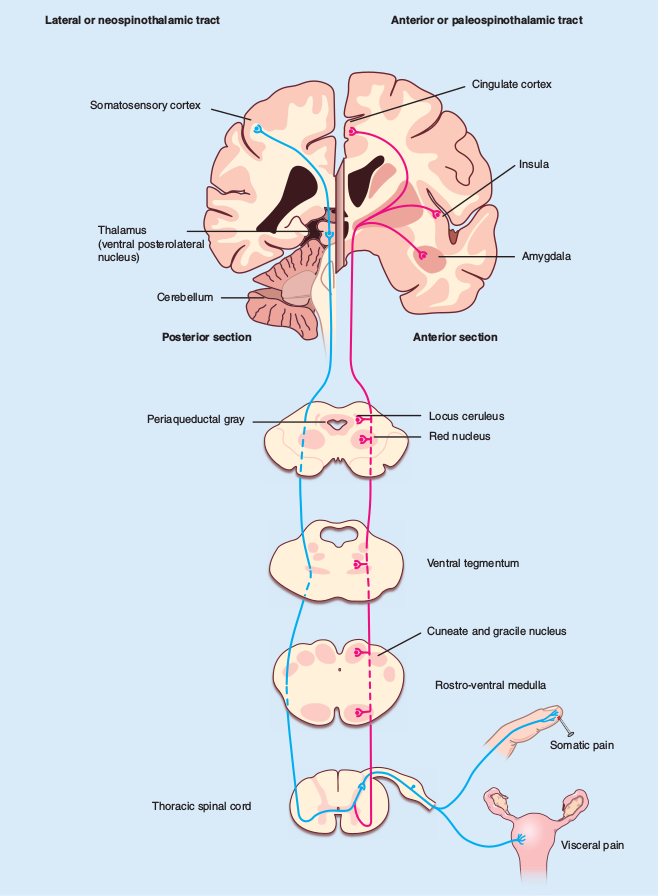
\includegraphics[width=1 \textwidth]{figures/PNG/Fenton2015.png}
 \caption{Nociception begins in the periphery and ascends toward the central nervous systems.
 Different nuclei along this path have the potential to down-regulate or suppress ascending signals. Similarly each of these locations (either from a peripheral or central source) can become dysregulated, allowing the phenomena often referred as persistent or chronic pain. \citep[300]{fenton2015neurobiology}}
 \label{fig:painperception}
 \end{figure}




